\chapter[Literature Review]{Literature Review}

\section{Introduction}
Various \acrfull{spa} frameworks exist with different strenghts and weaknesses. In this literature review, the three most popular frameworks are compared against each other. Additonally, the background and history of "Vue.js" is illustrated. Finally, the notion of \acrfull{seo} and the problem of acquiring a high search engine rank for \acrshort{spa}s is introduced and possible solutions are outlined.

\section{Comparison of SPA Frameworks}
As there is an excessive amount of libraries and frameworks available for creating web based applications this section will be limited to comparing Vue to the other most popular frameworks React and Angular. The following aspects of these will be evaluated: basic usage, scaling, performance, build size and ease of learning. As some terms are prone to ambiguity further clarification is necassary: basic usage describes how a framework is typically used when integrated into an environment that allows some kind of build process. For example Webpack is most commonly used as a bundler, providing a build process which main purpose it is to consolidate, transform and transpile code for usage in a browser, allowing developers to use next-gen JavaScript syntax that is not yet widely available in browsers among other things. Scaling discusses the capabilities of adding functionality to a framework. Flexibility describes if a framework enforces specific conventions in other words, how opionionated it is.
% VUE

\subsection{Vue 2.6.X}
Vue.js is considered a very performant JavaScript framework that "makes it easier for developers to create rich, interactive websites" \cite{macrae2018vue}. Instead of directly updating a site's \gls{DOM} which is an expensive operation Vue utilizes a virtual DOM \cite{ComparisonVue:online} - the representation of the actual DOM as a JavaScript object \cite{WhatIsVirtualDom:online}. When updating the UI, changes are made to this object which is a far cheaper operation. To get the real DOM in sync an efficient updating function is called, resulting in reduced ineffeciency especially in case many nodes have to be updated \cite{WhatIsVirtualDom:online}.

\subsubsection{Basic Usage} \label{subsub:vueusage}
 By default, any valid HTML can be used to define the basic structure of Vue components, which is also referred to as a "template" in Vue terminology. Component-scoped data and logic are defined within script tags and are complemented by functional directives such as "v-if" inside the template. Style sheets are defined within style tags, separating style and logic. By optionally using the scoped keyword, CSS is bound to a specific component, reducing the risk of polluting global style sheets. The composition of template, script and style tags is called a "Single File Component", indicating that only a single file is needed to create a functional and styled component. Additionally, props provide a uni-directional way of passing data from a parent component to a child component, whereas events are commonly used to pass data in the opposite direction. "Methods" can be defined to execute repeatable code, \gls{computed} "are calculations that will be cached based on their dependencies and will only update when needed" \cite{filipova2016learning} and \gls{watchers} which "watch" developer-defined properties and run a function everytime the property's value changes. \newline

\begin{lstlisting}[caption=Vue Single File Component, captionpos=b, style=htmlcssjs]{Vue Single File Component}
<template>
<div>
<h1 v-if="condition" class="custom-title"> Hello {{ user }} </h1>
<h1 v-else> "Hello Stranger" </h1>
</div>
</template>

</script>
export default {
    data: {
        return() {
            user: "Alex"
        }
    },
    methods: {/*execute code*/},
    computed: {/*return data when data changes*/},
    watch: {/*execute code when data changes*/}
}
</script>

</style scoped>
.custom-title {
    size: 30px;
}
</style>
\end{lstlisting}

\subsubsection{Scaling}
Vue applications can easily be scaled up or down in terms of application functionality depending on the requirements. In order to create sophisticated and large applications, three parts have to be incorporated in general: The core library, \gls{routing} and \gls{statemanagement}, of which all are officially provided by Vue as supporting libraries \cite{ComparisonVue:online}. This typically goes along with bundling tools such as Webpack or Browserify, which make for a much more powerful development environment. In addition, Vue offers an optional CLI generator interface for scaffolding projects, leaving the choice to the developer which building system and plugins to use. Using this interface, sophisticated applications along with routing and state management can be created. If the goal is to add reactive and interactive elements to an existing webpage, Vue can be used by adding a script tag to any valid site where necessary \cites{AddingReact:online, ComparisonVue:online}. In doing so, no bundler is needed for code to function but at the same time developers are deprived from being able to use plugins, preprocessors, and various other tools and are most commonly left with a larger bundle size \cite{ComparisonVue:online}.

\subsubsection{Performance \& Build Size}
The source size of Vue with the additional dependencies of vuex (\gls{statemanagement}) and vue-router is about ~30KB \cite{ComparisonVue:online}. As for performance, Vue is a very performant and efficient framework in terms of startup time, memory allocation and rendering time when compared to other technologies \cite{FrameworksPerformance:online}. Early beta versions of Vue 3.0 even reduce memory allocation and rendering time by about 50\%.

\subsubsection{Flexibility \& Learning Curve}
Among other things, Single File Components are easy to use when coming from an HTML background, make transitioning existing applications to Vue smoother, do not have a steep learning curve resulting in faster adoption by beginners and can be further enhanced with various preprocessors \cite{ComparisonVue:online}. As Vue supports various bundlers and build systems while not enforcing specific ways of usage, you could argue that it is less opinionated than some other technologies. 

% REACT

\subsection{React 16.8.X}

\subsubsection{Basic Usage}
React describes itself as a "library for building user interfaces" \cite[p.~2]{LearningReactBanks:book}. By using the word "library" it is implied that less functionality is shipped as opposed to using a traditional framework \cite[p.~2]{LearningReactBanks:book}. Like Vue it also utilizes a virtual DOM \cite[p.~81]{LearningReactBanks:book}. In React everything is defined in terms of JavaScript, meaning HTML often coupled with CSS are directly embedded into so called render functions. \acrfull{jsx}, which is essentially a syntax extension to JavaScript with XML-like features \cite{ReactJSX:online} is most commonly used (even though not necessary) to define these render functions and is capable of mixing the full power of a programming language with rendering and UI logic \cite{ComparisonVue:online}. Styling is most commonly achieved by CSS-in-JS solutions provided by additional libraries, effectively consolidating logic and styling in the same place \cite{islam2017reactjs:article}. \newline

\begin{lstlisting}[caption=Usage of JSX Render Function, captionpos=b, style=htmlcssjs]{Usage of JSX Render Function}
class Welcome extends React.Component {
    render() {
        return <h1>Hello, {this.props.name}</h1>;
    }
}
\end{lstlisting}

In addition, JSX render functions provide full leverage of JavaScript, including temporary variables and direct references to these and good tooling support (linting, type checking, autocompletion) \cite{ComparisonVue:online, ReactJSX:online}.

\subsubsection{Scaling}
Like Vue React can either be used with a bundler or added to a single site by using a script tag. React outsources \gls{routing} and \gls{statemanagement} to the community, fragmenting its ecosysytem in the process \cite{ComparisonVue:online}. More than eleven well-known routing libraries are available for React with similar statistics for \gls{statemanagement} and styling which gives developers a vast variety of available options but also makes choosing the right library for a projects requirements a much more tedious task. Reacts cli "create-react-app" works in a similar fashion like Vues but is much more limited: instead of letting the user choose a variety of options, it assumes that a single page application is to be created with always the same dependencies. However, an existing project can be migrated to a more customized environment with a command provided by React.

\subsubsection{Performance \& Build Size}
The React source itself has about 4.7KB gzipped which makes sense, given that React advertises itself as a library rather than a framework. However, including React DOM (34KB), \gls{routing} with react-router (6.9KB) and \gls{statemanagement} with redux (2.4KB) the total size grows considerably to 48KB. Performancewise, React is also very efficient when compared to other technologies, in fact, very similar to Vue \cite{FrameworksPerformance:online}. The reason for this, is mainly due to the usage of a virtual DOM.

\subsubsection{Flexibility \& Learning Curve}
To take advantage of online resources and documentation \acrshort{jsx} is almost a requirement. As it is an extension to JavaScript, developers who are familiar with this programming language can easily learn the additional syntax \cite{ReactJSX:online}. Without prior knowledge of JavaScript however, the learning curve rises considerably. At the same time, the availability of hundreds, perhaps even thousands of supporting libraries makes React very flexible, given that its core is so slim and additional functionality can easily be added by leveraging these. 

% ANGULAR
\subsection{Angular 7.2.X}

\subsubsection{Basic Usage}
Even though JavaScript could be used, Angular essentially requires the usage of TypeScript, a typed superset of JavaScript \cite{TypeScript:online}. As opposed to JavaScript, TypeScript comes with static type checking which naturally makes applications less prone to errors \cite{DynamicallyTypedLanguages:proceedings} and therefore is often used within very large corporate projects. Like Vue Angular also uses a component-based approach for composing user interfaces, but rather than using a single file, multiple files for HTML, CSS and JavaScript logic are typically created. \newline

\begin{lstlisting}[caption=Angular Basic Usage Example, captionpos=b, style=htmlcssjs]{Angular Basic Usage}
//app.component.html
<button (click)="show = !show">{{show ? 'hide' : 'show'}}</button> show = {{show}}
<br>
<div *ngIf="show; else elseBlock">Text to show</div>
<ng-template #elseBlock>Alternate text while primary text is hidden</ng-template>

// app.component.ts
import { Component } from '@angular/core';

@Component({
  selector: 'app-root',
  templateUrl: './app.component.html',
  styleUrls: ['./app.component.css']
})

export class SampleComponent {
  show: boolean = true;
}
\end{lstlisting}

\subsubsection{Scaling}
Designed with the purpose of building large and complex applications Angulars API exposes a lot of functionality which is most commonly only necessary for exactly these types of applications. It includes everything from routing, state management, http calls to complete testing suites, however, Angular can also be added to existing sites using a script tag, only providing core functionality.

\subsubsection{Performance \& Build Size}
Angular applications built with the angular project scaffolding interface angular-cli have around 65KB gzipped, double the space as the other two frameworks. As for performance, Angular is also a performant framework \cite{FrameworksPerformance:online} but becomes slow under certain circusmstances: For instance if a project utilizes a lot of watchers and data in the scope changes, all watchers are re-evaluated again \cite{ComparisonVue:online}.

\subsubsection{Flexibility \& Learning Curve}
 Angulars very big ecosystem and API provide most needed functionality out of the box but at the same time limit its flexibility. What is more, by prodiving pre-defined ways of interacting with Angular, it inherently becomes opinionated and more difficult to master \cite{ComparisonVue:online}.


\subsection{Conclusion}
% USAGE
All three frameworks solve similar problems but are used in different ways. Vues Single File Components consolidate logic, styles and HTML in the same place, React can and is most often used in a very resemblant way if used with a CSS-in-JS approach, whereas the "Angular way" is to split these parts into separate files. 

% SCALING
Applications built with React or Vue can be easily scaled up or down depending on the application-requirements. Large applications typically need the core library, routing and state management. While all of these are officially provided by the Vue core team for Vue applications, React leaves routing and state management to the community \cite{ComparisonVue:online}. Vue and React both offer an optional CLI generator interface to scaffold projects, however, Vue offers more options, leaving the choice to the developer which building system and plugins to use. React's more limiting approach with create-react-app makes it easier to start a project as it only needs a single dependency but limits the user to a given setup, which can however, be moved to a more customized environment with little effort whereas Angular is completely set up for the development of very large projects and provides most functionality out of the box, scaling up is therefore not a big problem because developers can rely on most of the functionality already existing.

All three frameworks can be scaled down by adding script tags to any site \cite{AddingReact:online, ComparisonVue:online} which however removes the powerful building layer.

% PERFORMANCE & BUILD SIZE
Vue and React both are similar in terms of runtime performance, are based on a virtual DOM and are used for similar use cases while Angular is a much more heavy-weight framework regarding performance and size. 

% FLEXIBILITY & LEARNING CURVE
JSX as well as TypeScript are additional learning steps and can lead to decreased productivity in smaller projects. Being a dynamic language, JavaScript's ability to address quickly changing requirements makes it especially suitable for rapid prototyping \cite[p.~72]{DynamicallyTypedLanguages:proceedings}. By using very HTML-like components Vue is often easier to master than the other two frameworks as most developers have at least basic knowledge of HTML. Nonetheless, Vue makes it possible to use TypeScript if the need arises, paving the way for bigger projects \cite{VueTypeScript:online}. Angular is not very flexible in the sense that users can pick whatever supporting library they deem best and is said to be an opinionated framework which enforces the "Angular way". Such frameworks are "pragmatic, with a strong sense of direction" \cite{Bedell:Opinionated:article} often forcing very specific conventions upon its users, effectively restricting what a developer can to with a framework. This also means there is a steeper learning curve but once overcome, can lead to increased productivity \cite{ComparisonVue:online}.

% Kiviat Diagram
The diagram shown in \autoref{fig:comparison} does by no means reflect the properties of the given framework / library 100\% accurately as some of them are somewhat subjective (e.g flexibility) but shall rather illustrate the strengths and weaknesses in relation to another when used in a typical manner.

\newcommand\ColorBox[1]{\textcolor{#1}{\rule{2ex}{2ex}}}

\begin{figure}[H]
\begin{center}
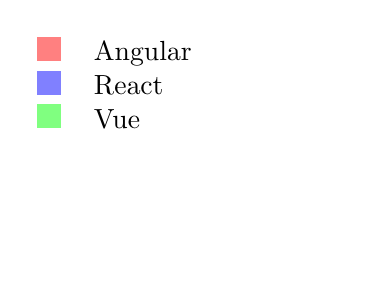
\begin{tikzpicture}
\tkzKiviatDiagram[scale=0.7,label distance=.5cm, radial=5, gap=1, lattice=5]
{Ease of Learning,Scaling,Performance,Compactness,Flexibility}
\tkzKiviatLine[thick, color=green, mark=none, fill=green!20, opacity=.5](5,3,4,4,3.5)
\tkzKiviatLine[thick, color=blue, mark=none, fill=blue!20, opacity=.5](4,4,3,3,4) 
\tkzKiviatLine[thick, color=red, mark=none, fill=red!20](2,5,2.5,1,2)    
% \tkzKiviatGrad[prefix=,unity=100,suffix=\ \texteuro](1)  
\node[anchor=south west,xshift=-60pt,yshift=40pt] at (current bounding box.south east) 
{
\begin{tabular}{@{}lp{3cm}@{}}
\ColorBox{red!50} & Angular \\
\ColorBox{blue!50} & React \\
\ColorBox{green!50} & Vue \\
\end{tabular}
};
\end{tikzpicture}
\end{center}
\caption{Comparison of Vue, React and Angular}
\label{fig:comparison}
\end{figure}

\section{Background of Vue.js}
% Talk about single page frameworks and how and why they were used and where to fell short of
Although existing frameworks were already used in order to create \acrlong{spa}, a concept which was discussed as early as 2003 \cite{Innerbro19:online} and used as a term for describing webinterfaces with a smooth almost native-like user experience \cite{Mikowski:Powell:2013}, none of these were designed with the purpose of rapidly prototyping UI interfaces. Angular, already widely used by developers and initially created by Google was too big and bloated of a framework to be sensible for small applications. React, a fairly new framework at the time also proved being too complex just like Backbone.js which was used for large-scale enterprise applications. There was something missing: a lightweight framework flexible enough to quickly build prototypes while not being too hard to master. As existing solutions did not seem adequate for this exact purpose \cite[p.~10]{filipova2016learning} new frameworks emerged, with Vue being one of them. Its lightweight approach of reactive data-binding and reusable HTML-based components helped fill that niche. Rising in popularity over the years Vue is now utilized for complex enterprise-grade applications and small prototpyes alike and has since been adopted by many developers and companies around the world. The most noteworthy of which are: Facebook, Netflix, Adobe, Xiaomi, Alibaba and GitLab \cite{CompaniesUsingVue:online}. With more than 130,000 stars on GitHub at the time of this writing, Vue is more popular than both React (122,000 stars) and Angular (45,000 stars).

\section{SEO for Single Page Applications} \label{sec:seo}

\subsection{Introduction}
There is no doubt that competing companies all over the world want to be found first in the biggest market of all: the internet. As 67.60\% of organic clicks are accounted by the first five pages returned by the SERP \cite{Khan2018:article}, these same companies are highly incentivized to invest into an improved search engine rank which was found to have a positive impact on an organizations performance \cite{yang2015search:article}. Therefore, the process of Search Engine Optimisation has become ubiquitous in our modern era as it promises to attract more users to a certain website \cite{Khan2018:article}. In other words: more users mean there is a greater probability of conversions, thus generating more revenue.

Unfortunately, successfully implementing SEO is a very delicate matter. In reality it is a set of techniques geared towards software rather than humans. These programs are commonly referred to as crawlers or bots which traverse the Web by exploiting the Web's hyperlinked structure and add their findings to the search engine's index \cite{Fink2014:inbook,menczer2001evaluating:proceedings}. They start on a websites root page and try to find any available links on that site \cite{Fink2014:inbook}. The process of choosing which links to follow, itself is dependant on complex algorithms as different crawlers will have to make different decisions \cite{menczer2001evaluating:proceedings}. For example a crawler trying to index the web as comprehensively as possible will have different underlying instructions than one that tries to find product reviews \cite{menczer2001evaluating:proceedings}. After being added to the index, a site's content is destructured and with additional metrics such as speed, size of images and mobile-friendliness its search engine rank is calculated \cite{Fink2014:inbook}.

Search Engine Optimisation helps crawlers better understand a site's content and "serves as a solution to figure out the nature of each webpage and determine how it can be made worthwhile to the users" \cite{Khan2018:article}.

\subsection{The Problem}
In general there are two ways to improve any type of site's rank: on-site optimisation and off-site optimisation \cite{Khan2018:article}. The first pertains to techniques that can be implemented on a site itself, such as efficiency of a webserver, compression of data, deferred loading of images, keywoards or the actual content, whereas the latter is a set of techniques which primarily drive more traffic to a certain site, such as social media marketing or the creation of backlinks \cite{Khan2018:article}. 

Improving a \acrlong{spa}'s ranking score proves difficult when using on-site optimisation techniques. When Google first started crawling websites in 1998 JavaScript was not a big problem as it was not widely used, so it simply was not executed \cite{GoogleUsesJavascript:online}. The rapidly changing landscape of webdesign however, demanded a more sophisticated approach. Things started to change drastically in 2014 when Google's crawler began executing JavaScript \cite{GoogleUsesJavascript:online}. However, as websites increasingly rely on AJAX \cite[p.~97]{Brunelle2016:article}, more specifically the deferred loading of resources, crawlers faced with a problem. The research of Brunelle et al. \cite[p.~97]{Brunelle2016:article} illustrates it as following:

\begin{quotation}
When a crawler fetches a web page (1), it waits for the page and all of the embedded resources to load to consider it fully rendered. At this point, the crawler preserves (2) all of the content on the web page (A). After the page has loaded, the page can request further resources (3), even without user interaction. The resource is then returned to the web page to be rendered (4) producing the final intended result (Ab). Because the crawler preserved the page prior to the page being fully loaded, the secondary content is not preserved and the archived version of the web page is not complete.
\end{quotation}

This can be seen as one of the biggest disadvantages for \acrshort{spa}'s as they heavily rely on AJAX and client-side rendering. If crawlers are not aware of their contents they will in turn suffer from a decreased search engine rank. 

\subsection{Possible Solutions} \label{sub:seo}
The problem is to be solved by offering crawlers a fully rendered page instead of having them load additional resources. This concept is called \acrfull{ssr} in broad terms. Depending on a web application's usage several variatons are feasible:

% Prerendering
\subsubsection{Prerendering}
The first is to implement prerendering: a process in which static HTML-files are created for specific routes at build time \cite{VueSSR:online}. This technique is especially useful for sites with content that does not change very often. Typical scenarios would be to create static versions of marketing or about sites \cite{VueSSR:online}. One of the main advantages is a rather simple setup process since creating a static version happens only once during building. At the same time, it becomes obvious that this solution is not very suitable for pages with rapidly changing content - rebuilding a project after every data change is not very efficient after all.

% SSR - Advantages and Disadvantages
\subsubsection{Server Side Rendering} \label{subsub:ssr}
A more sensible approach for sites with often changing content is \acrfull{ssr}. As opposed to prerendering, \acrshort{ssr} is a lot more sophisticated and complex to set up as it requires a tight coupling to the used framework. Upon every request by a client, the framework is responsible for creating a static version of the site which reflects the current available data. In technical terms, a static HTML site is rendered on the server by the framework, sent to the browser and hydrated "into a fully interactive app on the client" \cite{VueSSR:online}.

% Dynamic Rendering
\subsubsection{Dynamic Rendering}
Another possible solution which is still relevant today is to "create a static representation of your web site/application and direct crawlers to use it" and was identifed by Fink et al. in 2014 \cite[p.~270]{Fink2014:inbook}. This technique has been given the name "Dynamic Rendering" by Google in 2018 \cite{DynamicRenderingGoogle:online}. It differs from prerendering and SSR in on key aspect: real users and crawlers are served alternative content, hence the term "dynamic". When a crawler requests a site, an intermediate service transforms HTML and JavaScript to a static, prerendered version. This intermediate step allows for the creation of prerendered sites whenever needed - it builds upon prerendering but removes its build time constraint.


\subsubsection{Evaluation}
Prerendering is fairly easy to implement but is not very suitable for web applications with content that changes rapidly. As prerendering happens at build time, a project would have to be built every time content changes - an automated environment could be set up which builds the project after a given time interval, in this case however, it is noteworthy to mention that building is a rather expensive operation which takes longer the bigger the project is and deployment could result in downtime which accumulates over time. A better solution would be to use dynamic rendering, which builds upon prerendering but is run as a separate service, therefore coming with the benefits but not the disadvantages of normal prerendering. The most sophisticated approach and most complex to implement is \acrshort{ssr} which requires intimiate knowledge of a frameworks internals. However, there are solutions that take away some of that overhead for specific frameworks. Examples would be "Next.js" for React and "Nuxt.js" for Vue but in general, the previous statements apply. 